\documentclass[a4paper, 11pt, oneside]{article}

\usepackage[utf8]{inputenc}
\usepackage[T1]{fontenc}
\usepackage[english]{babel}
\usepackage{array}
\usepackage{shortvrb}
\usepackage{listings}
\usepackage[fleqn]{amsmath}
\usepackage{amsfonts}
\usepackage{fullpage}
\usepackage{enumerate}
\usepackage{graphicx}
\usepackage{alltt}
\usepackage{indentfirst}
\usepackage{eurosym}
\usepackage{titlesec, blindtext, color}
\usepackage[table,xcdraw,dvipsnames]{xcolor}
\usepackage[unicode]{hyperref}
\usepackage{url}
\usepackage{float}
\usepackage{subcaption}
\usepackage[skip=1ex]{caption}
\usepackage{dsfont}

\definecolor{brightpink}{rgb}{1.0, 0.0, 0.5}

\usepackage{titling}
\renewcommand\maketitlehooka{\null\mbox{}\vfill}
\renewcommand\maketitlehookd{\vfill\null}

\newcommand{\ClassName}{INFO8011: Network Infrastructures}
\newcommand{\ProjectName}{Software-Defined Networking in Data Centers}
\newcommand{\AcademicYear}{2021 - 2022}

%%%% First page settings %%%%

\title{\ClassName\\\vspace*{0.8cm}\ProjectName\vspace{1cm}}
\author{Maxime Goffart \\180521 \and Olivier Joris\\182113}
\date{\vspace{1cm}Academic year \AcademicYear}

\begin{document}

%%% First page %%%
\begin{titlingpage}
{\let\newpage\relax\maketitle}
\end{titlingpage}

\thispagestyle{empty}
\newpage

%%%%%%%%%%%%%%%%%%%%%%%%%%%%%%%%%%%%%%%%%%

\section{General overview}

\subsection{Spanning Tree Controller}
\paragraph{}This controller, as requested, builds a spanning tree in order to handle cycles in the network. To implement this solution, we first needed to discover the topology of the network. To do so, we used the functions \texttt{get\_host}, \texttt{get\_link}, and \texttt{get\_switch} of Ryu.\\
Then, based on the discovered topology, we built a graph of the topology where the vertices are the switches and the edges are the links between the switches. Afterwards, to compute the minimal spanning tree, we used Prim's algorithm.\\
\indent When packets are received at the controller, through \texttt{switch\_in\_handler} method, we check the source and the destination of each packet.\\
If the source is one of the host and the destination is broadcast, we broadcast the packet to the switches connected to the one that received it in the minimal spanning tree. Thus, the switches to which we sent the packet will send the packet to the controller that will, once again, do the same processing. At the same time, we set flows in the different switches so the controller will be contacted only once for a particular type of packets and it will reduce the RTT for similar requests.\\
If the source and the destination are both hosts, we compute a path between them using a depth-first search algorithm. Of course, the path is limited to links in the minimal spanning tree. When the path is computed, we set flows in the switches along the path so the controller will be contacted only once for a particular type of packets and it will reduce the RTT for similar request.


\subsection{Using VLANs}
\paragraph{}The implementation of this controller is based on the one of the spanning tree. Everything explained in the previous section is valid except that we are now separating the traffic into VLANs.
\paragraph{}This controller is building VLANs by mapping each port of the switches to one or several VLANs. This distribution is represented in figure \ref{VLANs_rep} which has been adapted from the picture given in the project statement. It is composed of 4 VLANs and the main idea is that each of the four core switches is responsible of the traffic corresponding to one VLAN. 
Only hosts belonging to the same VLAN can communicate with each other and the broadcast domain is also limited to this VLAN.

\begin{figure}[H]
    \center
    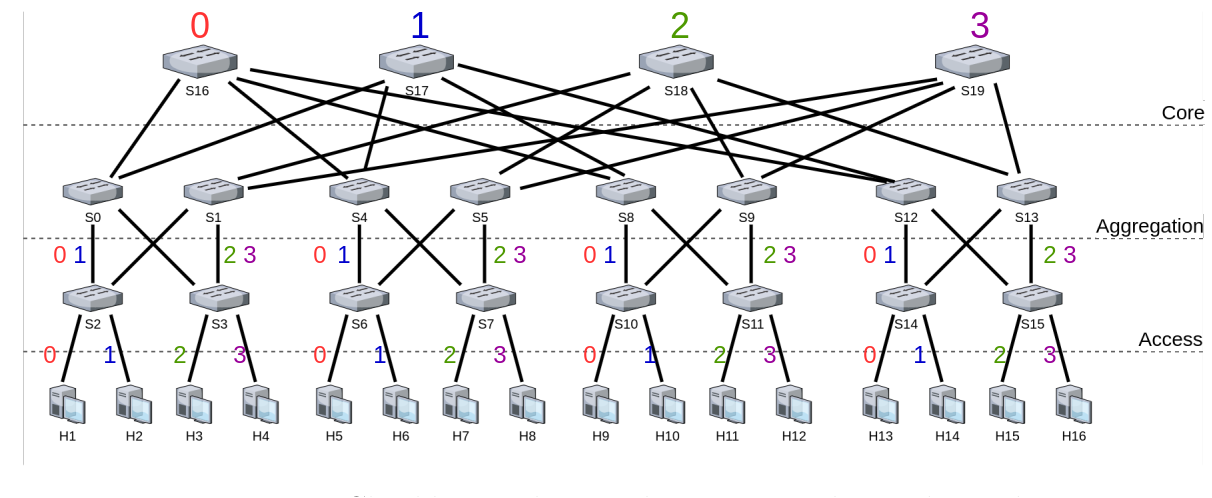
\includegraphics[scale = 0.4]{VLANs/VLANs.png}
    \caption{Map between links and VLANs.}
    \label{VLANs_rep}
    \end{figure}

\subsection{Adaptive routing} \label{subsec:adaptive}
\paragraph{}Unfortunately, we were not able to implement this controller. The reason is that we are supposed to use \texttt{OFPPortStatsRequest}, but, when we listen for the response, \texttt{EventOFPPortStatsReply}, in an handler, the reponse is always empty. Here is a screenshot of the execution of the code on one of our machine:
\begin{figure}[H]
\centering
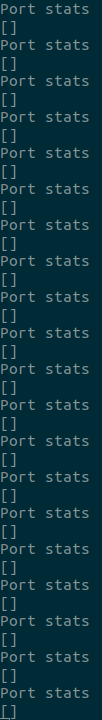
\includegraphics[scale=0.3]{port_stats.png}
\end{figure}
Thus, the file \texttt{adaptive.py} is just a copy of \texttt{spanningtree.py} with the code to handle \texttt{OFPPortStatsRequest} that always provides an empty response.

%%%%%%%%%%%%%%%%%%%%%%%%%%%%%%%%%%%%%%%%%%

\section{Tests}

\subsection{Spanning Tree Controller}
\subsubsection{Tests in normal conditions}
\paragraph{}If we ping 10 times each host from \texttt{h0}, we obtained the results of table \ref{table:STCPings}. The simple commands used are available in the file \texttt{test\_spanning\_tree.sh}.\\
\begin{table}[H]
\centering
\begin{tabular}{|l|l|l|l|}
\hline
\multicolumn{1}{|c|}{\textbf{Source-Dest}} & \multicolumn{1}{c|}{\textbf{Mean}} & \multicolumn{1}{c|}{\textbf{MDEV}} & \multicolumn{1}{c|}{\textbf{1st ping}} \\ \hline
H1-H2                                      & 272ms                              & 201ms                              & 877ms                                 \\ \hline
H1-H3                                      & 466ms                              & 124ms                              & 840ms                                 \\ \hline
H1-H4                                      & 460ms                              & 124ms                              & 830ms                                 \\ \hline
H1-H5                                      & 695ms                              & 192ms                              & 1274ms                                 \\ \hline
H1-H6                                      & 693ms                              & 188ms                              & 1258ms                                 \\ \hline
H1-H7                                      & 691ms                              & 208ms                              & 1317ms                                 \\ \hline
H1-H8                                      & 707ms                              & 198ms                              & 1300ms                                 \\ \hline
H1-H9                                      & 715ms                              & 210ms                              & 1347ms                                 \\ \hline
H1-H10                                      & 707ms                              & 200ms                              & 1306ms                                 \\ \hline
H1-H11                                     & 703ms                              & 200ms                              & 1300ms                                 \\ \hline
H1-H12                                     & 678ms                              & 192ms                              & 1256ms                                 \\ \hline
H1-H13                                     & 705ms                              & 181ms                              & 1247ms                                 \\ \hline
H1-H14                                     & 640ms                              & 15ms                              & 649ms                                 \\ \hline
H1-H15                                     & 694ms                              & 197ms                              & 1287ms                                 \\ \hline
H1-H16                                     & 701ms                              & 200ms                              & 1302ms                                 \\ \hline
\end{tabular}
\caption{Results of 10 pings between each host and \texttt{h0}}
\label{table:STCPings}
\end{table}
We can see that the first ping always take a lot of time. This is explained because the first ping we will have as consequence to send multiple packets to the controller. First, it will send packets to the controller related to the ARP request to learn the MAC address of the destination. Then, it will send packets to the controller related to the icmp messages which will require the computation of paths between the host and the destination. All the processing in the controller is done in Python which is well known to be a slow language. Furthermore, these tests were performed on Maxime's computer which had the vm lock with an execution cap at 10\% (see in section \ref{sec:feedback} the explanation).\\
Yet, the pings, after the first one of each test, have a RTT around the mean value. The high values of MDEV are explained by the fact that the first ping take a lot of time thus it increases the values of MDEV.\\
Another reason for the high value is the fact that each link has a delay of 50ms as set in the Mininet topology provided. Finally, we should keep in mind that we are running in a virtual environment and not on physical devices thus the measurements are not the most precise. Also, real physical links would not have a delay of 50ms (except for very long distance).

\paragraph{}If we measure the bandwidth between \texttt{Source} and \texttt{Dest}, we obtain the results expressed in table \ref{table:ST_bw}. We can observe that, when the distance between the host is increasing, the bandwidth is decreasing which is logical because more switches have to be traversed inside the spanning tree. Moreover, if we perform multiple \texttt{iperf} from multiple hosts at the same time, the bandwidth is decreasing more.

\begin{table}[H]
    \centering
    \begin{tabular}{|l|l|l|}
    \hline
    \textbf{Source-Dest} & \textbf{Min}   & \textbf{Max}   \\ \hline
    H1-H2                & 2.13 Mbits/sec & 2.5 Mbits/sec  \\ \hline
    H1-H3                & 1.02 Mbits/sec & 1.31 Mbits/sec \\ \hline
    H1-H4                & 923 Kbits/sec  & 1.21 Mbits/sec \\ \hline
    H1-H5                & 670 Kbits/sec  & 871 Kbits/sec  \\ \hline
    H1-H6                & 670 Kbits/sec  & 870 Kbits/sec  \\ \hline
    H1-H7                & 671 Kbits/sec  & 872 Kbits/sec  \\ \hline
    H1-H8                & 623 Kbits/sec  & 872 Kbits/sec  \\ \hline
    H1-H9                & 622 Kbits/sec  & 870 Kbits/sec  \\ \hline
    H1-H10               & 671 Kbits/sec  & 969 Kbits/sec  \\ \hline
    H1-H11               & 663 Kbits/sec  & 872 Kbits/sec  \\ \hline
    H1-H12               & 670 Kbits/sec  & 792 Kbits/sec  \\ \hline
    H1-H13               & 670 Kbits/sec  & 870 Kbits/sec  \\ \hline
    H1-H14               & 669 Kbits/sec  & 969 Kbits/sec  \\ \hline
    H1-H15               & 671 Kbits/sec  & 872 Kbits/sec  \\ \hline
    H1-H16               & 669 Kbits/sec  & 869 Kbits/sec  \\ \hline
    \end{tabular}
    \caption{Results of iperf between \texttt{Source} and \texttt{Dest}}
    \label{table:ST_bw}
    \end{table}


\subsubsection{Tests when a switch/link fails}
\paragraph{}First, we can try to ping \texttt{h5} from \texttt{h1} and \texttt{h15} from \texttt{h1}. Both pings work as expected. Now, let us simulate a switch failure by typing \texttt{switch s17 stop} in Mininet. Then, ping \texttt{h5} from \texttt{h1} and \texttt{h15} from \texttt{h1}. Both work because our controller react to the change of topology. Now, let us simulate the switch going back up by typing \texttt{switch s17 start} in Mininet and do the same 2 pings as before. Both work because our controller react to the change of topology.\\
This simple test is available in the file \texttt{test\_spanning\_tree\_failure.sh}.

\subsection{Using VLANs}
The commands used to performed these tests are available in the \texttt{test\_vlans.sh} script.
\subsubsection{Reachability}

\paragraph{}The reachability can be verified using the \texttt{pingall} command which give the output represented on the figure \ref{VLANs_reach}. We observe that hosts can communicate with each other only if they belong to the same VLAN.

\begin{figure}[H]
\center
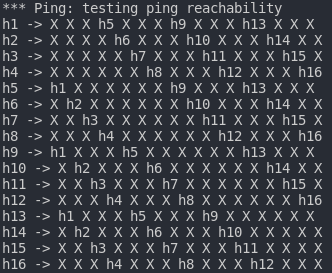
\includegraphics[scale = 2]{VLANs/VLANs_reach.png}
\caption{Reachability of hosts using VLANs.}
\label{VLANs_reach}
\end{figure}

\subsubsection{Measures}

\paragraph{}If we ping 10 times from \texttt{Source} to \texttt{Dest}, we obtain the results of table \ref{table:VLANs_pings}. We observe that the measures are quite similar for each VLAN which is logical because all VLANs are distributed with the same number of switches and hosts. 
\begin{table}[H]
    \centering
    \begin{tabular}{|l|l|l|l|}
    \hline
    \multicolumn{1}{|c|}{\textbf{Source-Dest}} & \multicolumn{1}{c|}{\textbf{Mean}} & \multicolumn{1}{c|}{\textbf{MDEV}} & \multicolumn{1}{c|}{\textbf{1st ping}} \\ \hline
    H1-H5                                      & 671ms                              & 210ms                              & 1301ms                                 \\ \hline
    H1-H9                                      & 666ms                              & 188ms                              & 1229ms                                 \\ \hline
    H1-H13                                      & 664ms                              & 188ms                              & 1229ms                                 \\ \hline
    H2-H6                                      & 664ms                              & 187ms                              & 1225ms                                 \\ \hline
    H2-H10                                      & 662ms                              & 184ms                              & 1215ms                                 \\ \hline
    H2-H14                                     & 663ms                              & 188ms                              & 1229ms                                 \\ \hline
    H3-H7                                      & 668ms                              & 200ms                              & 1268ms                                 \\ \hline
    H3-H11                                      & 664ms                              & 186ms                              & 1223ms                                 \\ \hline
    H3-H15                                      & 664ms                              & 187ms                              & 1227ms                                 \\ \hline
    H4-H8                                    & 670ms                              & 208ms                              & 1294ms                                 \\ \hline
    H4-H12                                     & 662ms                              & 184ms                              & 1216ms                                 \\ \hline
    H4-H16                                     & 664ms                              & 189ms                              & 1232ms                                 \\ \hline
    \end{tabular}
    \caption{Results of 10 pings between \texttt{Source} and \texttt{Dest}}
    \label{table:VLANs_pings}
    \end{table}

\paragraph{}If we measure the bandwidth between \texttt{Source} and \texttt{Dest}, we obtain the results expressed in table \ref{table:VLANs_bw}. We observe that the measures are quite similar for each VLAN which is logical for the same reason as for the measures relative to ping. These measures stay stable when combining \texttt{iperf} from different hosts of different VLANs at the same time which is the principal interest to use this controller rather than the spanning tree controller.
\begin{table}[H]
    \centering
    \begin{tabular}{|l|l|l|}
    \hline
    \textbf{Source-Dest} & \textbf{Min}  & \textbf{Max}   \\ \hline
    H1-H5                & 621 Kbits/sec & 791 Kbits/sec  \\ \hline
    H1-H9                & 670 Kbits/sec & 872 Kbits/sec  \\ \hline
    H1-H13               & 669 Kbits/sec & 872 Kbits/sec  \\ \hline
    H2-H6                & 670 Kbits/sec & 871 Kbits/sec  \\ \hline
    H2-H10               & 670 Kbits/sec & 872 Kbits/sec  \\ \hline
    H2-H14               & 667 Kbits/sec & 873 Kbits/sec  \\ \hline
    H3-H7                & 667 Kbits/sec & 872 Kbits/sec  \\ \hline
    H3-H11               & 670 Kbits/sec & 871 Kbits/sec  \\ \hline
    H3-H15               & 721 Kbits/sec & 1.03 Mbits/sec \\ \hline
    H4-H8                & 671 Kbits/sec & 872 Kbits/sec  \\ \hline
    H4-H12               & 663 Kbits/sec & 871 Kbits/sec  \\ \hline
    H4-H16               & 621 Kbits/sec & 870 Kbits/sec  \\ \hline
    \end{tabular}
    \caption{Results of iperf between \texttt{Source} and \texttt{Dest}}
    \label{table:VLANs_bw}
    \end{table}
\subsection{Adaptive routing}
\paragraph{}As explained in section \ref{subsec:adaptive}, we were not able to implement this controller. Thus, there is nothing to test.

%%%%%%%%%%%%%%%%%%%%%%%%%%%%%%%%%%%%%%%%%%

\section{Feedback} \label{sec:feedback}
\subsection{Main difficulties}
\paragraph{}We encountered multiple difficulties when working on this assignment. Here is a list of the difficulties we encountered:
\begin{itemize}
\item Instabilities of the virtual machine, Mininet, and Ryu. For instance, Maxime had to cap the execution of the processor for the virtual machine at 10\% or the code would not work. He lost some time trying to understand the issue. An other example is what we experienced in section \ref{subsec:adaptive}.
\item Most documentations, even the official book, on how to use Ryu is for OpenFlow 1.3 while we were blocked to OpenFlow 1.0. The differences between the 2 versions are minors but they are resulting in lose time that could be used to improve our understanding of SDN. Also regarding documentations, they are not always very well done.
\end{itemize}
These difficulties have the consequence that we have the impression that we spent more time on details related to Ryu and different versions of OpenFlow than really improving our understanding of SDN. Furthermore, these difficulties increased the difficulty of the project uselessly.

\subsection{Time spent on the project}
Olivier spent approximately 17 hours working on the project while Maxime did unfortunately not keep track of the time he spent working on the project.

\subsection{Possible improvements}
\paragraph{}Here is a list of possible improvements for the project:
\begin{itemize}
\item Switching to OpenFlow 1.3 because, as mentioned previously, most documentations on Ryu are using OpenFlow 1.3 and we will not lose time on details related to which version of OpenFlow we are using.
\item Maybe using something else than Ryu because we had issues related to it (e.g. needing to cap the execution of the processor or some functions of Ryu would return anything).
\end{itemize}

%%%%%%%%%%%%%%%%%%%%%%%%%%%%%%%%%%%%%%%%%%
\end{document}